\documentclass{beamer}
\usetheme{Madrid}
\usecolortheme{default}

\usepackage[utf8]{inputenc}
\usepackage[T1]{fontenc}
\usepackage{listings}
\usepackage{xcolor}
\usepackage{booktabs}
\usepackage{amssymb}

\definecolor{codegray}{gray}{0.5}
\definecolor{codeblue}{rgb}{0.0,0.0,0.6}
\lstdefinestyle{verilog}{
  language=Verilog,
  basicstyle=\ttfamily\scriptsize,
  keywordstyle=\color{codeblue}\bfseries,
  commentstyle=\color{codegray}\itshape,
  numbers=none,
  breaklines=true,
  showstringspaces=false,
}
\lstset{style=verilog}

\title[RISC-V Pipeline + RVC]{Procesador RISC-V Pipelined con Extensión C}
\subtitle{Pipeline, Hazard Unit e Instrucciones Comprimidas}
\author[Ildefonso, Paucar, Rosillo]{%
  \begin{tabular}[t]{c}Ildefonso Santos\\Steve Andy\end{tabular}
  \and
  \begin{tabular}[t]{c}Paucar Barrios\\Miguel Luis\end{tabular}
  \and
  \begin{tabular}[t]{c}Rosillo Rodríguez\\Marcelo Mateo\end{tabular}
}
\institute{UTEC --- Arquitectura de Computadoras}
\date[]{Julio 2026}

\makeatletter
\setbeamertemplate{footline}{%
  \leavevmode%
  \hbox{%
  \begin{beamercolorbox}[wd=.5\paperwidth,ht=2.25ex,dp=1ex,center]{author in head/foot}%
    \usebeamerfont{author in head/foot}\insertshortauthor
  \end{beamercolorbox}%
  \begin{beamercolorbox}[wd=.5\paperwidth,ht=2.25ex,dp=1ex,leftskip=5em,rightskip=1ex]{title in head/foot}%
    \usebeamerfont{title in head/foot}\insertshorttitle\hfill
    \insertframenumber{} / \inserttotalframenumber
  \end{beamercolorbox}}%
  \vskip0pt%
}
\makeatother

\AtBeginSection[]
{
  \begin{frame}
    \frametitle{Contenido}
    \tableofcontents[currentsection]
  \end{frame}
}

\begin{document}

\frame{\titlepage}

\begin{frame}{Contenido}
  \tableofcontents
\end{frame}

% ============================================================
\section{Pipeline y Hazard Unit}
% ============================================================

\begin{frame}{El pipeline base: 5 etapas}
  \begin{columns}
    \column{0.55\textwidth}
    \begin{itemize}
      \item<1-> \textbf{Fetch}: PC, memoria de instrucciones
      \item<2-> \textbf{Decode}: banco de registros, extend
      \item<3-> \textbf{Execute}: ALU, cálculo de saltos
      \item<4-> \textbf{Memory}: memoria de datos
      \item<5-> \textbf{Writeback}: escritura al banco de registros
    \end{itemize}
    \column{0.45\textwidth}
    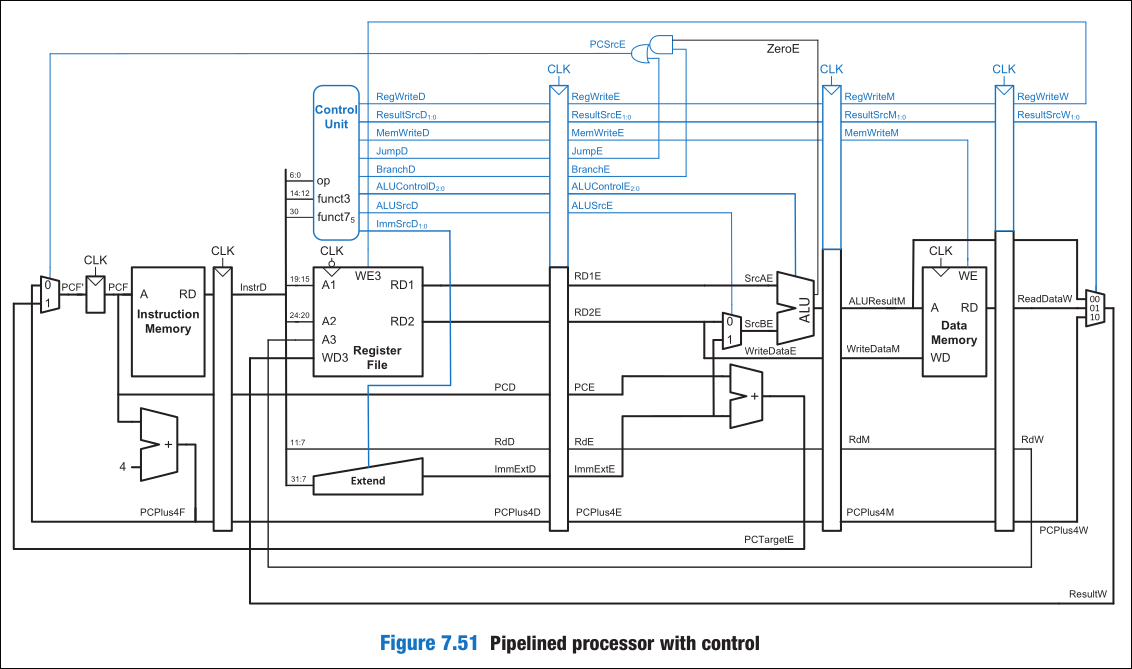
\includegraphics[width=\textwidth]{../pipeline_diagram.png}
  \end{columns}
\end{frame}

\begin{frame}{Riesgos (\textit{hazards})}
  \begin{block}{El precio de segmentar}
    Varias instrucciones en vuelo a la vez $\Rightarrow$ los datos y saltos no
    siempre están listos a tiempo.
  \end{block}
  \begin{itemize}
    \item \alert{De datos (RAW)}: una instrucción usa un resultado que otra
      anterior aún no escribió. Caso crítico: \textit{load-use}.
    \item \alert{De control}: los saltos se resuelven en Execute, pero ya se
      captaron instrucciones secuenciales de más.
    \item \alert{Estructurales}: evitados por diseño (imem/dmem separadas,
      regfile lee y escribe en el mismo ciclo).
  \end{itemize}
\end{frame}

\begin{frame}{Sin unidad de riesgos: los programas fallan}
  \begin{columns}
    \column{0.5\textwidth}
    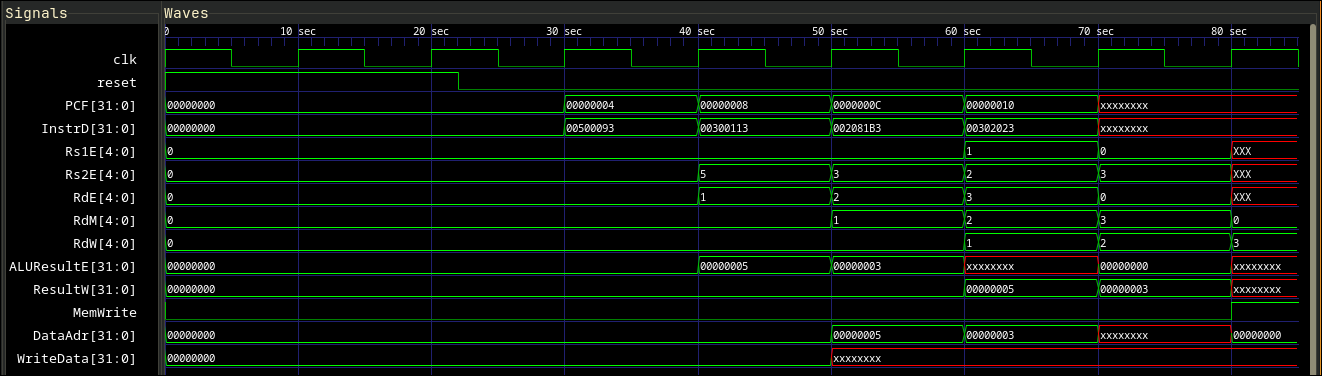
\includegraphics[width=\textwidth]{../hazard_forward_nohu.png}
    \column{0.5\textwidth}
    \begin{itemize}
      \item \texttt{add x3,x1,x2} lee \texttt{x1}/\texttt{x2} \textbf{antes}
        de que se escriban en Writeback.
      \item \texttt{ALUResultE} sale en \texttt{X}.
      \item El dato corrupto llega hasta \texttt{WriteData}.
    \end{itemize}
  \end{columns}
\end{frame}

\begin{frame}{Solución: \textit{forwarding}, \textit{stall}, \textit{flush}}
  \begin{itemize}
    \item<1-> \textbf{Forwarding}: adelanta el resultado desde EX/MEM o
      MEM/WB directo a la ALU (\texttt{ForwardAE/BE}).
    \item<2-> \textbf{Stalling}: detiene Fetch/Decode un ciclo en el caso
      \textit{load-use} (\texttt{StallF/D}).
    \item<3-> \textbf{Flushing}: descarta instrucciones mal captadas tras un
      salto tomado (\texttt{FlushD/E}).
  \end{itemize}
  \vspace{0.3cm}
  \begin{exampleblock}{Resultado}
    Los mismos tres programas (forward, stall, flush) \textbf{pasan}
    correctamente con la hazard unit activa.
  \end{exampleblock}
\end{frame}

\begin{frame}{Datapath final: implementación de instrucciones}
  \centering
  \includegraphics[width=0.98\textwidth]{../datapath_final.pdf}
  \vspace{2mm}

  {\scriptsize En \textcolor{red}{rojo}: adiciones propias sobre el pipeline
  base --- \texttt{Jalr}, \texttt{funct3E}, \texttt{ALUControl} de 4 bits,
  mux de destino \texttt{jalr}.}
\end{frame}

% ============================================================
\section{Extensión C: instrucciones comprimidas}
% ============================================================

\begin{frame}{¿Qué es RVC?}
  \begin{itemize}
    \item Instrucciones de \textbf{16 bits} que coexisten con las de 32 bits.
    \item Reducen el tamaño del código \textbf{25--30\,\%} sin perder
      expresividad.
    \item Cada comprimida tiene \textbf{exactamente un} equivalente de 32 bits.
  \end{itemize}
  \begin{alertblock}{Estrategia: descomprimir en Fetch}
    Expandir los 16 bits a RV32I \textbf{antes} del registro IF/ID. Decode,
    Execute, Memory, Writeback, \texttt{controller}, \texttt{hazardunit}
    \textbf{no se modifican}.
  \end{alertblock}
\end{frame}

\begin{frame}[fragile]{Cambios en el datapath}
  \begin{enumerate}
    \item \textbf{Ventana deslizante} en \texttt{imem}: una comprimida puede
      dejar al PC desalineado a palabra.
\begin{lstlisting}
assign rd = a[1] ? {w1[15:0], w0[31:16]} : w0;
\end{lstlisting}
    \item \textbf{Incremento variable}: \texttt{PC += compressed ? 2 : 4}.
    \item \textbf{Módulo \texttt{decompressor.v}}: combinacional, produce la
      instrucción expandida antes del IF/ID.
  \end{enumerate}
  \begin{block}{Costo en ciclos}
    \textbf{Cero.} Todo es combinacional dentro de la etapa Fetch.
  \end{block}
\end{frame}

\begin{frame}{Módulos agregados / afectados}
  \begin{center}
  \small
  \begin{tabular}{@{}ll@{}}
    \toprule
    \textbf{Módulo} & \textbf{Rol} \\
    \midrule
    \texttt{decompressor.v} & Nuevo. Expande 16$\to$32 bits (combinacional) \\
    \texttt{imem.v} & Ventana deslizante para PC desalineado \\
    \texttt{datapath.v} & \texttt{PCPlusInc}, instancia del decompressor \\
    \texttt{alu.v} & +5 operaciones: xor, lui, sll, srl, sra \\
    \bottomrule
  \end{tabular}
  \end{center}
  \vspace{3mm}
  \centering
  \textbf{Sin cambios:} \texttt{controller}, \texttt{extend}, \texttt{regfile},
  \texttt{hazardunit}, \texttt{dmem}
\end{frame}

\begin{frame}{ALU modificada}
  \centering
  \includegraphics[width=0.85\textwidth]{../alu_modificada.pdf}

  {\scriptsize \textcolor{red}{Rojo}: \texttt{xor}, \texttt{lui}, y el
  \textit{shifter} (\texttt{sll}/\texttt{srl}/\texttt{sra}). Mux de salida
  creció de 5 a 10 entradas; \texttt{ALUControl} de 3 a 4 bits.}
\end{frame}

\begin{frame}[fragile]{Las 21 instrucciones comprimidas}
  \footnotesize
  \begin{columns}
    \column{0.5\textwidth}
    \textbf{Parte 1 (E2) --- 11 instr.}
    \begin{itemize}
      \item CI: \texttt{c.addi, c.lui, c.slli}
      \item CR: \texttt{c.add}
      \item CA: \texttt{c.sub, c.xor, c.or, c.and}
      \item CB: \texttt{c.srli, c.srai, c.andi}
    \end{itemize}
    \column{0.5\textwidth}
    \textbf{Parte 2 (E3) --- 10 instr.}
    \begin{itemize}
      \item CL/CS: \texttt{c.lw, c.sw}
      \item CI/CSS: \texttt{c.lwsp, c.swsp}
      \item CB: \texttt{c.beqz, c.bnez}
      \item CJ: \texttt{c.j, c.jal}
      \item CR: \texttt{c.jr, c.jalr}
    \end{itemize}
  \end{columns}
\end{frame}

\begin{frame}[fragile]{Ejemplo: \texttt{c.lw} / \texttt{c.sw}}
  Registros restringidos \texttt{x8--x15}, \textit{offset} de 7 bits
  \textbf{barajado} (\textit{scrambled}):
\begin{lstlisting}
wire [6:0] offlw = {c[5], c[12:10], c[6], 2'b00};

5'b00_010: instr = {5'b0, offlw, rs1p, 3'b010,
                     rs2p, 7'b0000011};              // c.lw
5'b00_110: instr = {5'b0, offlw[6:5], rs2p, rs1p,
                     3'b010, offlw[4:2], 2'b00,
                     7'b0100011};                    // c.sw
\end{lstlisting}
  \alert{Bug detectado y corregido}: el destino de \texttt{c.lw} vive en
  \texttt{c[4:2]} (formato CL), no en \texttt{c[9:7]} --- se confunde
  fácilmente con \texttt{rs1'}.
\end{frame}

\begin{frame}[fragile]{Ejemplo: desambiguación \texttt{c.jr}/\texttt{c.jalr}/\texttt{c.add}}
  Comparten \texttt{\{op,funct3\}=\{10,100\}} (formato CR) junto con
  \texttt{c.mv} (subproducto de la desambiguación, no requerido). Se
  distinguen con \texttt{c[12]} y si \texttt{rs2} es cero:
\begin{lstlisting}
if (!c[12] && rs2 == 5'b0)
  instr = {12'b0, rd, 3'b000, 5'b00000, 7'b1100111}; // c.jr
else if (!c[12])
  instr = {7'b0, rs2, 5'b00000, 3'b000, rd, 7'b0110011}; // c.mv
else if (rs2 == 5'b0)
  instr = {12'b0, rd, 3'b000, 5'b00001, 7'b1100111}; // c.jalr
else
  instr = {7'b0000000, rs2, rd, 3'b000, rd, 7'b0110011}; // c.add
\end{lstlisting}
  \begin{center}
  \small
  \begin{tabular}{@{}cccl@{}}
    \toprule
    \texttt{c[12]} & \texttt{rs2=0?} & \textbf{Instrucción} & \textbf{Expande a} \\
    \midrule
    0 & sí & \texttt{c.jr} & \texttt{jalr x0, rs1, 0} \\
    1 & sí & \texttt{c.jalr} & \texttt{jalr x1, rs1, 0} \\
    1 & no & \texttt{c.add} & \texttt{add rd, rd, rs2} \\
    \bottomrule
  \end{tabular}
  \end{center}
\end{frame}

\begin{frame}[fragile]{Encoding de las 21 instrucciones}
  \tiny
  \begin{columns}
    \column{0.5\textwidth}
    \begin{tabular}{@{}llll@{}}
      \toprule
      \textbf{Instr.} & \textbf{op} & \textbf{f3} & \textbf{Fmt} \\
      \midrule
      \texttt{c.addi} & 01 & 000 & CI \\
      \texttt{c.jal}  & 01 & 001 & CJ \\
      \texttt{c.lui}  & 01 & 011 & CI \\
      \texttt{c.srli} & 01 & 100 & CB \\
      \texttt{c.srai} & 01 & 100 & CB \\
      \texttt{c.andi} & 01 & 100 & CB \\
      \texttt{c.sub}  & 01 & 100 & CA \\
      \texttt{c.xor}  & 01 & 100 & CA \\
      \texttt{c.or}   & 01 & 100 & CA \\
      \texttt{c.and}  & 01 & 100 & CA \\
      \texttt{c.j}    & 01 & 101 & CJ \\
      \texttt{c.beqz} & 01 & 110 & CB \\
      \bottomrule
    \end{tabular}
    \column{0.5\textwidth}
    \begin{tabular}{@{}llll@{}}
      \toprule
      \textbf{Instr.} & \textbf{op} & \textbf{f3} & \textbf{Fmt} \\
      \midrule
      \texttt{c.bnez} & 01 & 111 & CB \\
      \texttt{c.slli} & 10 & 000 & CI \\
      \texttt{c.lwsp} & 10 & 010 & CI \\
      \texttt{c.jr}   & 10 & 100 & CR \\
      \texttt{c.jalr} & 10 & 100 & CR \\
      \texttt{c.add}  & 10 & 100 & CR \\
      \texttt{c.swsp} & 10 & 110 & CSS \\
      \texttt{c.lw}   & 00 & 010 & CL \\
      \texttt{c.sw}   & 00 & 110 & CS \\
      \bottomrule
    \end{tabular}
  \end{columns}
  \vspace{2mm}
  \small\centering \texttt{op = c[1:0]}, \texttt{funct3 = c[15:13]}
\end{frame}

\begin{frame}{Limitaciones de RVC}
  \begin{itemize}
    \item \texttt{c.beqz}/\texttt{c.bnez} solo comparan contra \texttt{x0}: no
      existe compresión directa de \texttt{blt}/\texttt{bge}.
    \item \textit{Offsets} de memoria limitados: \texttt{c.lw}/\texttt{c.sw}
      hasta 124; superarlo obliga a materializar la dirección con
      instrucciones extra.
    \item Registros restringidos (\texttt{x8--x15}) en varios formatos:
      limita qué instrucciones se pueden comprimir según el registro usado.
  \end{itemize}
\end{frame}

% ============================================================
\section{Resultados: algoritmo y comparativa}
% ============================================================

\begin{frame}[fragile]{Programa algoritmo: \texttt{sumloop}}
  Bucle que acumula $5+4+3+2+1=15$, mezclando 32 y 16 bits:
\begin{lstlisting}
    addi x8, x0, 5     ; n = 5            (32 bits)
    addi x9, x0, 0     ; acc = 0          (32 bits)
LOOP:
    add  x9, x9, x8    ; c.add: acc += n  (16 bits)
    addi x8, x8, -1    ; c.addi: n--      (16 bits)
    bnez x8, LOOP      ; c.bnez: repetir  (16 bits)
    sw   x9, 0(x0)     ; Mem[0] = 15      (32 bits)
\end{lstlisting}
\end{frame}

\begin{frame}{Waveform del algoritmo}
  \centering
  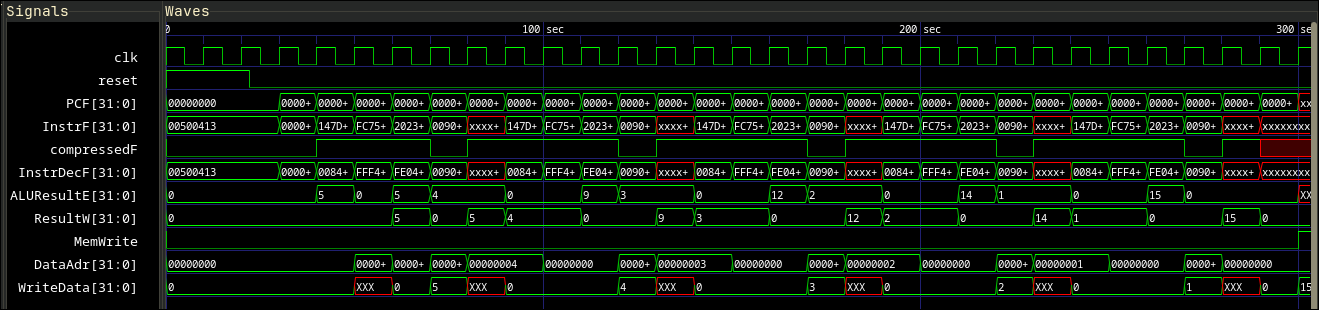
\includegraphics[width=\textwidth]{../sumloop_waveform.png}
  {\scriptsize \texttt{PCF} itera $0x8{\to}0xA{\to}0xC{\to}0x8$;
  \texttt{ALUResultE} acumula $5,9,12,14,15$.}
\end{frame}

\begin{frame}{Comparativa: tamaño y \textit{performance}}
  \begin{table}
    \centering
    \small
    \begin{tabular}{@{}lccc@{}}
      \toprule
      \textbf{Versión} & \textbf{Instrucciones} & \textbf{Bytes} & \textbf{Reducción} \\
      \midrule
      RV32I puro & $6\times4$B & 24 & --- \\
      Con RVC & $3\times4$B $+$ $3\times2$B & 18 & \textbf{25\,\%} \\
      \bottomrule
    \end{tabular}
  \end{table}
  \begin{columns}
    \column{0.5\textwidth}
    \begin{block}{Tamaño}
      25\,\% menos código. En programas reales, 25--30\,\% típico.
    \end{block}
    \column{0.5\textwidth}
    \begin{alertblock}{\textit{Performance}}
      \textbf{Idéntico}: mismos ciclos, misma cantidad de instrucciones
      ejecutadas. La ventana deslizante no cuesta ciclos.
    \end{alertblock}
  \end{columns}
\end{frame}

\begin{frame}{Validación}
  \begin{center}
  \small
  \begin{tabular}{@{}lll@{}}
    \toprule
    \textbf{Categoría} & \textbf{Pruebas} & \textbf{Resultado} \\
    \midrule
    Pipeline base (E1) & 12 testbenches & \checkmark \\
    RVC Parte 1 (E2) & caddi, cir, ca, cb, mul10 & \checkmark \\
    RVC Parte 2 (E3) & clsw, clspsp, cbz, cj, cjr & \checkmark \\
    Algoritmo & sumloop & \checkmark \\
    \bottomrule
  \end{tabular}
  \end{center}
  \begin{center}
    \Large \textbf{23 / 23 PASS}
  \end{center}
\end{frame}

% ============================================================
\section{Conclusiones}
% ============================================================

\begin{frame}{Conclusiones, desafíos y mejoras}
  \begin{itemize}
    \item<1-> \textbf{Conclusión clave}: descomprimir en Fetch permite añadir
      todo un ISA nuevo \textbf{sin tocar} el pipeline ni la hazard unit.
    \item<2-> \textbf{Desafío principal}: los \textit{immediates} barajados
      (\textit{scrambled}) --- fácil confundir posiciones de bits entre
      formatos CL/CS/CB/CJ/CI/CSS.
    \item<3-> \textbf{Mejora a futuro}: soportar \textit{illegal instruction}
      trap para comprimidas mal formadas; extender a RV64C.
  \end{itemize}
\end{frame}

\begin{frame}
  \centering
  \Huge Gracias
  \vspace{1cm}

  \normalsize Preguntas
\end{frame}

\end{document}
